\documentclass{article}
\usepackage{algorithms_in_data_mining}

\begin{document} %
\lecture{11}{$k$-means clustering}{Edo Liberty}

\section{Introduction}
\begin{definition}[$k$-means]
Given $n$ vectors $x_1\ldots,x_n\in \R^d$, and an integer $k$, find $k$ points $\mu_1,\ldots,\mu_k \in \R^d$
which minimize the expression:
\[
f_{k-means} = \sum_{i \in [n]} \min_{j \in [k]} \|x_i - \mu_j \|^2
\]
\end{definition}
I words, we aim to find $k$ cluster centers. The cost is the squared distance between all the points to their closest cluster center.
k-means clustering and Lloyd's algorithm \cite{Lloyd82leastsquares} are probably the most widely used clustering procedure.
This is for three main reasons:
\begin{itemize} 
\item The objective function is simple and natural.
\item Lloyd's algorithm (which we see below) is simple, efficient and often results in the optimal solution.  
\item The results are easily interpretable and are often quite descriptive for real data sets. 
\end{itemize}
In 1957 Stuart Lloyd suggested a simple iterative algorithm which efficiently finds a local minimum for this problem.
This algorithm (a.k.a. Lloyd's algorithm) seems to work so well in practice that it is sometimes referred to as $k$-means or the $k$-means algorithm.

\begin{algorithm}
\caption{Lloyd's Algorithm}
\begin{algorithmic}
\STATE $\mu_1,\ldots,\mu_k \leftarrow$ randomly chosen centers
\WHILE {Objective function still improves}
\STATE $S_1,\ldots,S_k \leftarrow \phi$
\FOR {$i \in 1,\ldots,n$}
	\STATE $j \leftarrow \arg\min_{j'}\|x_i - \mu_{j'}\|^2 \}$
	\STATE add $i$ to $S_j$
\ENDFOR
\FOR {$j \in 1,\ldots,k$}
	\STATE $\mu_j = \frac{1}{|S_j|}\sum_{i \in S_j} x_i$
\ENDFOR
\ENDWHILE
\end{algorithmic}
\end{algorithm}
This algorithm can be thought of as a potential function reducing algorithm.
The potential function is 
\[
f_{k-means} = \sum_{j \in [k]} \sum_{i \in S_j} \|x_i - \mu_j\|^2.
\]
The sets $S_j$ are the sets of points to which $\mu_j$ is the closest center.
In each step of the algorithm the potential function is reduced.
Let's examine that.
First, if the set of centers $\mu_j$ are fixed, the best assignment is clearly the one which assigns
each data point to its closest center. Also, assume that $\mu$ is the center of a set of points $S$.
Then, if we move $\mu$ to $\frac{1}{|S|}\sum_{i \in S} x_i$ then we only reduce the potential.
This is because $\frac{1}{|S|}\sum_{i \in S} x_i$ is the best possible value for $\mu$ (can easily be seen by derivation of the cost function).

The algorithm therefore terminates in a local minimum.
The question of course is whether we can guaranty that the solution is close to optimal and under what computational cost.

\section{k-means and PCA}
This section will present a simple connection between $k$-means and PCA (similar ideas given here \cite{DingH04a}).
\begin{figure}[h!]
  \centering
  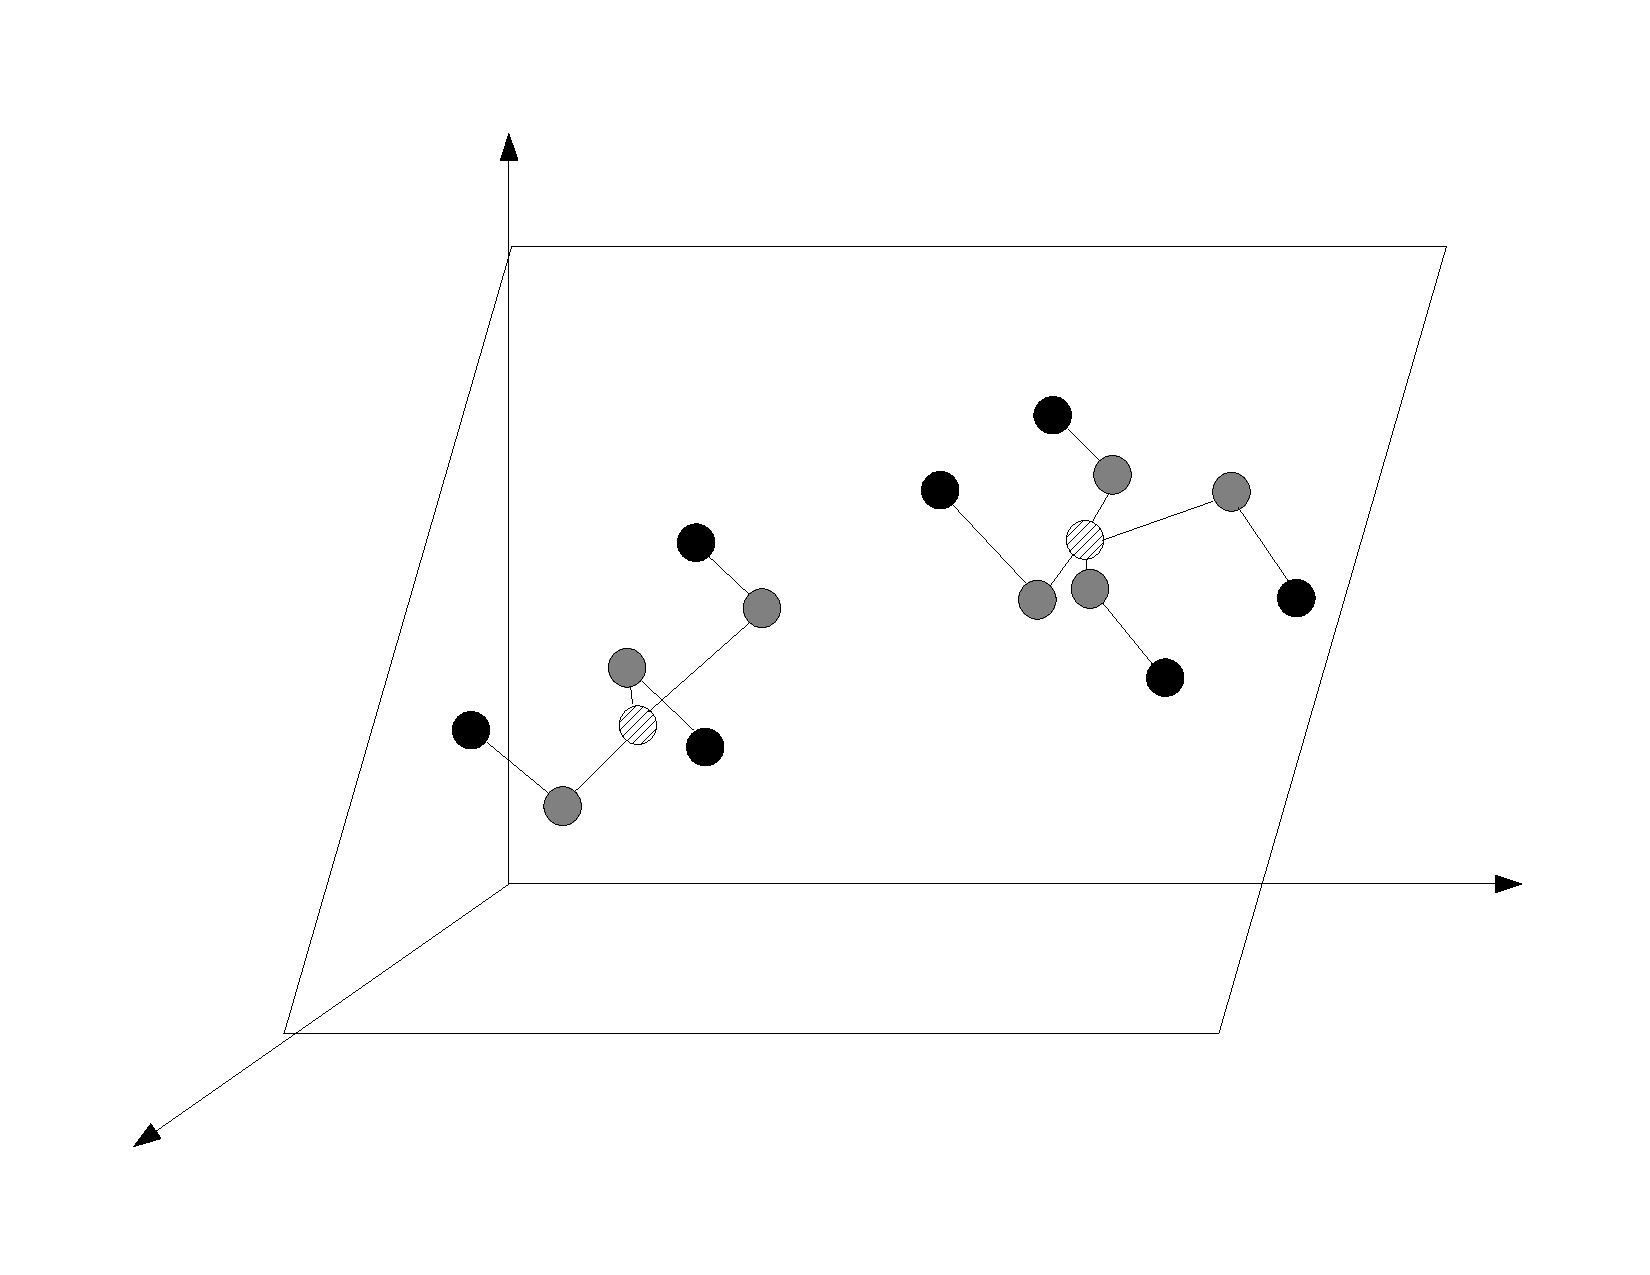
\includegraphics[width=0.6\textwidth]{11_images/PCA-kmeans.pdf}
  \caption{Example of $k$-means $(k=2)$ cost broken into a PCA cost and a $k$-means cost in dimension $k$.}
\end{figure}

First, consider the similarity between the $k$-means cost function
\[
f_{k-means} = \min_{\mu_1,\ldots,\mu_k} \sum_{i \in [n]} \min_{j \in [k]} \|x_i - \mu_j \|^2
\]
and that of PCA
\[
f_{PCA} = \min_{P_k} \sum_{i \in [n]} \|x_i - P_{k} x_i \|^2 = \min_{P_k} \sum_{i \in [n]} \min_{y_i \in P_k} \|x_i - y_i \|^2
\]
where $P_k$ is a projection into dimension $k$ and $y \in P_k$ means that $P_k y = y$.
The equality stems from the fact that for any point $x$ and projection matrix $P$ we have that $\arg\min_{y \in P} \|x - y\| = Px$.

Now, think about the subspace $P^{*}_{k}$ which contains the $k$ optimal centers. 
Since $\mu^{*}_{j} \in P^{*}_{k}$ we have that:
\begin{eqnarray}
f_{k-means} &=& \sum_{i \in [n]} \min_{j \in [k]} \|x_i - \mu^{*}_j \|^2 \\
&\ge& \sum_{i \in [n]} \min_{y_i \in P^{*}_{k}} \|x_i - y_i \|^2 \\
&\ge& \min_{P_{k}}\sum_{i \in [n]} \min_{y_i \in P_{k}} \|x_i - y_i \|^2 \\
&=&  \min_{P_{k}}\sum_{i \in [n]} \|x_i - P_k x_i \|^2 = f_{PCA}
\end{eqnarray}

Now, consider solving $k$-means on the points $y_i$ instead. This intuitively will be an easier task
because they are isometrically embedded into dimension exactly $k$ (by the projection $P_k$). 
Before we do that though, we should argue that a good clustering for $y_i$ results in a good clustering to $x_i$.
Let $P$ be any projection and let $y_i = Px_i$ and $\hat{\mu}_{j} = P{\mu}_{j}$. We have that:
\begin{eqnarray}
\sum_{j \in [k]} \sum_{i \in S_j}  \|x_i - \mu_j \|^2 &\ge& \sum_{j \in [k]} \sum_{i \in S_j}  \|Px_i - P\mu_j \|^2 \\
&\ge& \sum_{j \in [k]} \sum_{i \in S_j}  \|y_i - \hat{\mu}_{j}\|^2 \\
&\ge& \sum_{j \in [k]} \sum_{i \in \hat{S}_j}  \|y_i - \hat{\mu}_{j}\|^2 = \hat{f}_{k-means}
\end{eqnarray}
where $\hat{S}$ and $\hat{\mu}$ are the assignments and centers of the projected points $y_i$.


The following gives us a simple algorithm. Compute the $PCA$ of the points $x_i$ into dimension $k$.
Solve $k$-means on the points $y_i$ in dimension $k$. Output the resulting clusters and centers.
\begin{eqnarray}
f_{alg} &=& \sum_{j \in [k]} \sum_{i \in \hat{S}_j} \|x_i -\hat{\mu}_j \|^2 \\
&=& \sum_{j \in [k]} \sum_{i \in \hat{S}_j} \|x_i -y_i \|^2 + \|y_i - \hat{\mu}_j\|^2 \\
&= & \sum_{i \in [n]} \|x_i -y_i \|^2 + \sum_{j \in [k]} \sum_{i \in \hat{S}_j}\|y_i - \hat{\mu}_j\|^2 \\
&=& f_{PCA} + \hat{f}_{k-means} \le 2f_{k-means}
\end{eqnarray}

\subsection{$\eps$-net argument for fixed dimensions}
Since computing the SVD of a matrix (and hence PCA) is well known. 
We get that computing a $2$-approximation to 
the $k$-means problem in dimension $d$ is possible if it can be done in dimension $k$.

To solve this problem we adopt a brut force approach.
Let $Q_{\eps}$ be a set of points inside the unit ball $B^{k}_{1}$ such that:
\[
\forall z \in B^{k}_{1} \;\; \exists \; q \in Q_{\eps} \; s.t. \;\; \|z - q\| \le \eps
\]
Such sets of points exist such that  $|Q_{\eps}| \le c(\frac{1}{\eps})^k$. There are 
probabilistic constructions for such sets as well but we will not go into that.
Assuming w.l.o.g. that $\|x_i\| \le 1$ we can constrain the centers of 
the clusters to one of the points in the $\eps$-net $Q_{\eps}$.
Let $q_j$ be the closes point in $Q_{\eps}$ to $\mu_j$ (so $\|\mu_j - q_j \| \le \eps$).
From a simple calculation we have that:
\[
\sum_{j \in [k]} \sum_{i \in S_j} \|x_i - q_j \|^2 \le  \sum_{j \in [k]} \sum_{i \in S_j} \|x_i - \mu_j \|^2 + 5\eps.
\]
 
To find the best clustering we can exhaustively search through every set of $k$ points from $Q_{\eps}$.
For each such set, compute the cost of this assignment on the original points and return the one minimizing the cost.
That will require ${c(\frac{1}{\eps})^k \choose k}$ iterations over candidate solutions each of which requires $O(ndk)$ time. 
The final running time we achieve is $2^{O(k^2\log(1/\eps))}nd$. 


\section{Sampling}
Another simple idea is to sample sufficiently many points from the input as candidate centers.
Ideas similar to the ones described here can be found here \cite{ZhaHDGS01}.

First, assume we have only one set of points $S$. 
Also, denote by $\mu$ the centroid of $S$, $\mu = \frac{1}{\|S\|}\sum_{i \in S} x_i$.
We will claim that picking one of the members of $S$ as a centroid is not much worse than
picking $\mu$.
Let $q$ be a member of $S$ chosen uniformly at random.
Let us compute the expectation of the cost function.
\begin{eqnarray}
\E[\sum_{i \in S} \|x_i - q\|^2] &=& \sum_{i \in S} \sum_{j \in S} \frac{1}{n}\|x_i - x_j\|^2  \\
&\le& \sum_{i \in S} \sum_{j \in S} \frac{1}{n}\cdot2(\|x_j - \mu\|^2 + \|x_i - \mu\|^2) \\
&\le& 4 \sum_{i \in S}  \|x_i - \mu\|^2.
\end{eqnarray}

Using Markov's inequality we get that
\[
\Pr[\sum_{i \in S} \|x_i - q\|^2 \le 8\sum_{i \in S}  \|x_i - \mu\|^2] \ge 1/2
\]
If this happens we say that $q$ is a good representative for $S$.
Now consider again the situation where we have $k$ clusters $S_1,\dots,S_k$.
If we are given a set $Q$ which contains a good candidate for each of the sets.
Then, restricting ourselves to pick centers from $Q$ will result in at most a multiplicative factor of $8$ to the cost.

The set $Q$ can be quite small if the set are roughly balanced.
Let the smallest set contain $n_s$ points. 
We therefore succeed in finding a good representative for any set with probability at least $\frac{1}{2}\frac{n_s}{n}$.
The probability of failure for any set is thus bounded by $k (1 - \frac{n_s}{2n})^{|Q|}$.
Therefore $|Q| = O(k \log(k))$ if $n_s \in \Omega(n/k)$.

Again, iterating over all subsets of $Q$ of size $k$ we can find an approximate 
solution is time $O({ck \log(k) \choose k}knd) = 2^{O(k \log(k))}nd$.

\section{Advanced reading}

In the above, we gave approximation algorithms to the $k$-means problem.
Alas, any solution can be improved by performing Lloyds algorithm on its output.
Therefore, such algorithms can be considered as `seeding' algorithms 
which give initial assignments to Lloyds algorithm.
A well known seeding procedure \cite{ArthurV07} is called $k$-means++.
\begin{algorithm}
\caption{$k$-means++ algorithm  \cite{ArthurV07}}
\begin{algorithmic}
\STATE $C \leftarrow \{x_i\}$ where $x_i$ is a uniformly chosen from $[n]$.
\FOR{$j \in [k]$}
	\STATE Pick node $x$ with probability proportional to $\min_{\mu \in C} \|x - \mu\|^2$
	\STATE Add $x$ to $C$
\ENDFOR
\STATE {\bf return:} $C$
\end{algorithmic}
\end{algorithm}
In each iteration, the next center is chosen randomly from the input points.
The distribution over the points is not uniform. 
Each point picked with probability proportional to the minimal square distance from it to a picked center.
Surprisingly, This simple and practical approach already gives an $O(\log(k))$ approximation guarantee.
More precisely, let $f_{k-means}(C)$ denote the cost of $k$-means with the set of centers $C$.
Also, denote by $C*$ the optimal set of centers. Then 
\[
\E[f_{k-means}(C)] \le 8 (\log(k)+2).
\]

In \cite{AilonJM09} the authors give a streaming algorithm for this problem.
They manipulate ideas from \cite{ArthurV07} and combine them with a hirarchical 
divide and conquer methodology. See also \cite{GuhaMMMO03} for a thorough survey and
new techniques for clustering in streams.

Another problem which is very related to $k$-means is the $k$-medians problem.
Given a set to points $x_1,\ldots,x_n$ the aim is to find centers $\mu_1,\ldots,\mu_k$ which minimize:
\[
f_{k-medians} = \sum_{i \in [n]} \min_{j \in [k]} \|x_i - \mu_j \|
\]
Both $k$-means and the $k$-median problem admit $1+\eps$ multiplicative approximation algorithms but these
are far from being simple. See \cite{hk-sckmk-05} for more details, related work, and a new core set based solution. 


\bibliographystyle{plain}
\bibliography{algorithms_in_data_mining}
\end{document}

